\documentclass[]{article}

\usepackage{emoji}
\usepackage{graphicx}

\begin{titlepage}
    \title{IDATT2103, Øving 8}
    \author{Jakob Grønhaug (jakobkg@stud.ntnu.no)}
    \date{}
\end{titlepage}
\begin{document}
    \maketitle
    \section*{Case}
    I denne oppgaven har jeg valgt å lage en database-løsning relatert til jobben min, som kundestøtte for bedriftkunder hos et større selskap. Denne database-løsningen er tenkt som grunnlag for et saksbehandlings-system, der flere behandlere kan logge inn for å se, opprette eller redigere loggførte saker og saksdokumenter som er knyttet opp mot et gitt kundeforhold.

    I denne modellen vil det være nødvendig med tabeller for kundebehandlere, kundeforhold, saker, saksinnhold og sakstyper. Tabellen for kundebehandlere burde kunne unikt identifisere hver enkelt kundebehandler, men fremdeles gjøre det mulig å endre på ting som fornavn og etternavn da dette er informasjon som kan endre seg gjennom et ansettelsesfohold og ikke burde være låst i databasen. En god kandidatnøkkel kan være et ansattnummer, eller et unikt brukernavn. Tabellen med kundeforhold burde inneholde unike kundenumre, kunders navn og organisasjonsnummer, og en form for kobling som gjør det mulig å knytte flere saker i sakssystemet til samme kunde. Hver sak i sakssystemet må være tilknyttet en kunde og en kundebehandler, ha en tittel og en beskrivelse, en sakstype og et tidspunkt som angir når saken ble opprettet. Saker må også ha saksinnhold og en sakstype, der saksinnhold kan være ting som saksbehandlers notater, epost sendt til kunde og epost mottatt fra kunde, og sakstype vil være kategorier som "support", "klage", "salgshenvendelse" o.l.

    \subsection*{Kundebehandler}
    Relasjonen som beskriver en kundebehandler burde ha felter for unikt brukernavn (\emoji{old-key}), fornavn, etternavn, epost-adresse og team-tilhørighet.

    \begin{table}[ht]
        \centering
        \begin{tabular}{|c|c|c|}
            \hline
            \multicolumn{3}{|c|}{\textbf{Kundebehandler}} \\
            \hline
            Ansattnummer & integer & \emoji{old-key} \\
            \hline
            Fornavn & string &  \\
            \hline
            Etternavn & string & \\
            \hline
            Epost & string & \\
            \hline
            Team & integer & FK \\
            \hline
        \end{tabular}
    \end{table}

    \subsection*{Team}
    For å fordele saksbehandlere i team vil jeg også putte eksisterende team i en egen tabell, slik at hver behandler har en fremmednøkkel som peker til team-tabellen. På denne måten sikres det at man ikke ved et uhell feilstaver noens team slik at de ikke dukker opp ved et database-søk av typen "Finn alle saker som er behandletav Team 3", og om et team oppløses vil man bedre kunne gjøre flyttingen av saksbehandlere til andre team da databasen kan konfigureres til å feile slettingen av et team fra tabellen dersom en eller flere kundebehandlere fremdeles har en fremmednøkkel som peker til teamet som skal slettes.

    \begin{table*}[ht]
        \centering
        \begin{tabular}{|c|c|c|}
            \hline
            \multicolumn{3}{|c|}{\textbf{Team}} \\
            \hline
            ID & integer & \emoji{old-key} \\
            \hline
            Navn & string & \\
            \hline
        \end{tabular}
    \end{table*}

    \subsection*{Kundeforhold}
    I denne tenkte situasjonen er kundene i systemet andre bedrifter, dermed er både kundenummer og organisasjonsnummer potensielle hovednøkler. I tillegg burde bedriftens navn, adresse og kontaktinfo være registrert.

    \begin{table}[ht]
        \centering
        \begin{tabular}{|c|c|c|}
            \hline
            \multicolumn{3}{|c|}{\textbf{Kundeforhold}} \\
            \hline
            Kundenummer & integer & \emoji{old-key} \\
            \hline
            Org.-nummer & string &  \\
            \hline
            Navn & string &  \\
            \hline
            Adresse & string & \\
            \hline
            Epost & string & \\
            \hline
            Telefonnummer & string &  \\
            \hline
        \end{tabular}
    \end{table}

    \subsection*{Sak}
    Hver sak i systemet må ha et unikt saksnummer, være eid av en kundebehandler og være tilknyttet en bestemt kunde. I tillegg burde en sak ha et emne-felt, en beskrivelse og en kategori. En sak kan også inneholde flere forskjellige innlegg, som for eksempel kan være saksbehandlers notater, en mail sendt inn fra kunden eller en mail sendt ut til kunden. Siden en enkelt sak kan inneholde null til mange stykker med innhold vil ikke disse lagres i denne tabellen, men heller ved at hvert stykke innhold har saksnummeret som fremmednøkkel og kan finnes ved å søke i tabellene for innhold og filtrere på saksnummer-feltet.

    \begin{table}[ht]
        \centering
        \begin{tabular}{|c|c|c|}
            \hline
            \multicolumn{3}{|c|}{\textbf{Sak}} \\
            \hline
            Saksnummer & integer & \emoji{old-key} \\
            \hline
            Kunde & integer & FK \\
            \hline
            Saksbehandler & integer & FK \\
            \hline
            Emne & string &  \\
            \hline
            Beskrivelse & string & \\
            \hline
            Kategori & integer & FK \\
            \hline
        \end{tabular}
    \end{table}

    \pagebreak

    \subsection*{Saksinnhold}
    Hver sak kan inneholde null eller flere poster med innhold. For enkelhets skyld har jeg valg å holde disse til to typer, eposter og saksnotater. Disse puttes i hver sin tabell, og for å sikre at de kan vises i riktig rekkefølge for en saksbehandler har de også et dato-felt som de kan sorteres etter.

    \begin{table}[ht]
        \centering
        \begin{tabular}{|c|c|c|}
            \hline
            \multicolumn{3}{|c|}{\textbf{Notat}} \\
            \hline
            ID & integer & \emoji{old-key} \\
            \hline
            Saksnummer & integer & \\
            \hline
            Opprettet & date & \\
            \hline
            Forfatter & integer & FK \\
            \hline
            Innhold & string & \\
            \hline
        \end{tabular}
        \quad
        \begin{tabular}{|c|c|c|}
            \hline
            \multicolumn{3}{|c|}{\textbf{E-post}} \\
            \hline
            ID & integer & \emoji{old-key} \\
            \hline
            Saksnummer & integer & \\
            \hline
            Opprettet & date & \\
            \hline
            Fra & string &  \\
            \hline
            Til & string &  \\
            \hline
            Innhold & string & \\
            \hline
        \end{tabular}
    \end{table}

    \pagebreak

    \section*{ER-modell}
    \begin{figure}[h]
        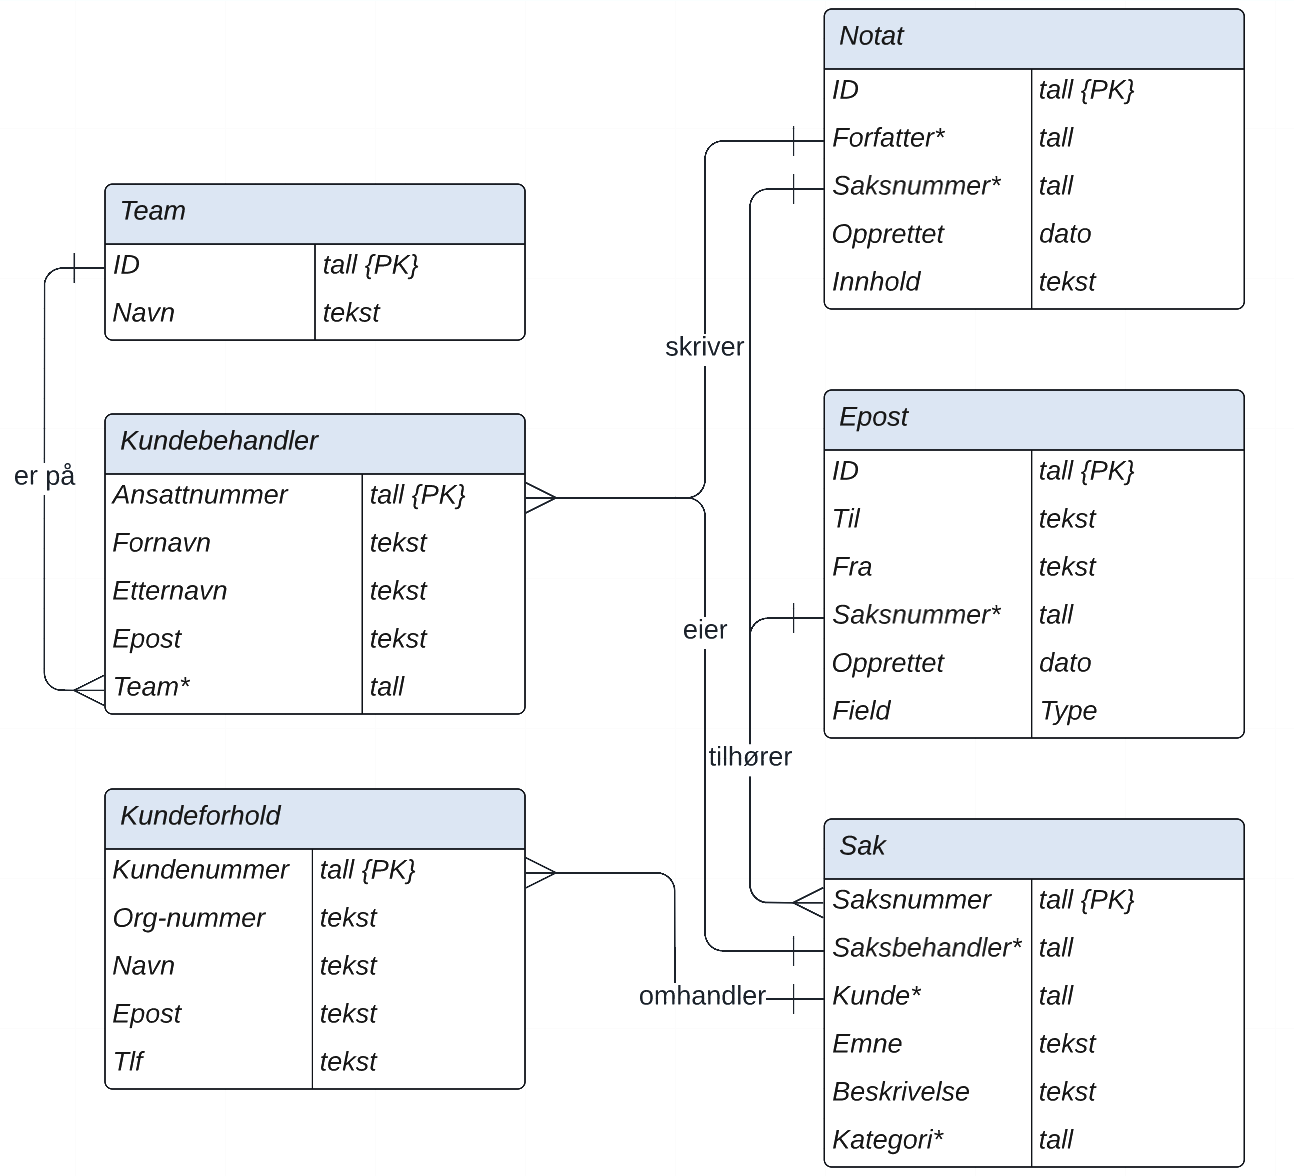
\includegraphics{er-diagram.png}
    \end{figure}

    \section*{Spørringer}

    \subsection*{Hent alle innlegg for visning av en sak}

    \begin{verbatim}
        select
            *
        from 
            sak
            natural join
            epost
            natural join
            notat
        where
            saksnummer = <ønsket saksnummer>;
    \end{verbatim}

    \subsection*{Finn alle saker behandlet av et gitt team}

    \begin{verbatim}
        select
            *
        from
            sak
            natural join
            kundebehandler
            natural join
            team
        where
            team.id = <ønsket team>;
    \end{verbatim}
    
    \subsection*{Finn ut hvem som har behandlet saker angående en kunde, om noen}

    \begin{verbatim}
        select
            saksbehandler.fornavn,
            saksbehandler.etternavn,
            sak.saksnummer
        from
            sak
            right join
            kundebehandler
            on sak.saksbehandler = kundebehandler.id
            right join
            kunde
            on kunde.kundenummer = sak.kunde
        where
            kunde.kundenummer = <ønsket kunde>;
    \end{verbatim}

    \subsection*{Oppsummering}

    Denne database-strukturen er relativt enkel, uten noen mellom-tabeller for null-til-mange-relasjoner. Det gjør den også heller snill å skrive spørringer mot, og jeg tror ikke jeg ville gjort noen ting nevneverdig annerledes med modellen jeg har per nå. Den er dog relativt liten, og kunne godt vært utvidet med flere tabeller som kan tilføre videre nytteverdi. Team kan ha teamledere, en kunde kan ha en eller flere kontaktpersoner i stedet for kun ett felt for kontaktinfo, og andre ting enn notater og eposter kan kanskje eksistere inne i saker?

    \section*{XML/JSON i MySQL}

    XML eller JSON brukes som regel for å lagre semi-strukturert data i en database, gjerne der strukturen på data kan endres etter behov. De mest aktuelle områdene å utforske dette på i database-løsningen beskrevet ovenfor vil være tabellene for saksinnhold, der det nå er separate tabeller for interne notater og for mail-korrespondanse. Her kunne det vært mulig med en datastruktur som dekker både disse tilfellene og eventuelt flere andre former for saksinnhold, definert i XML/JSON og integrert med teknologi som XQuery eller lignende. Dette gjør det også mulig å ha et egen-definert format på dataen som kan flyttes på tvers av programvareløsninger, slik at det er enklere å bytte saksbehandlingsverktøy enn om dataen er lagret i et proprietært format.

    Dermed kan tabellene for saksnotater og epost slås sammen til en "Innhold"-tabell som lagrer XML.

    \begin{table}[ht]
        \centering
        \begin{tabular}{|c|c|c|}
            \hline
            \multicolumn{3}{|c|}{\textbf{Innhold}} \\
            \hline
            ID & integer & \emoji{old-key} \\
            \hline
            Saksnummer & integer & FK \\
            \hline
            Tidspunkt & dato & \\
            \hline
            Innhold & XML & \\
            \hline
        \end{tabular}
    \end{table}

    Herfra kan man for eksempel hente brødteksten fra et stykke saksinnhold med en spørring som minner om

    \begin{verbatim}
        select
            ExtractValue(brødtekst, '/innlegg/brødtekst')
        as
            brødtekst
        from
            innhold;
    \end{verbatim}

    En slik løsning er dog ikke uten ulemper, som å kanskje konvertere mellom XML-formatet og saksbehandlingsverktøyets proprietære dataformat ved lagringi og lesning fra databasen. Det å introdusere en ny teknologi i en løsning vil også føre til økt terskel for å jobbe videre med databasen, mer tid som kreves for opplæring før evt. nye vedlikeholdere eller utviklere kan settes inn i prosjektet og en spredning av definisjoner for dataformat mellom SQL og JSON/XML.

    \section*{NoSQL-løsning}

    Siden denne løsningen er bygd som en relasjonsdatabase fra bunnen av tror jeg ikke den vil være lett overførbar til en NoSQL-løsning. Noen deler av den er lett å se for seg i NoSQL, for eksempel er tabellene om saker med beskrivelse, notater og andre innlegg en god kandidat for en dokumentdatabase. Å bruke en dokumentdatabase kan også bedre tilrettelegge for smidig utvikling der kravspesifikasjoner er flytende og kan endre seg gjennom utviklingsprosessen. Jeg er ikke like overbevist om at ting som listen over kunder og saksbehandlere vil vesentlig forbedres av å endre fra en SQL-basert løsning til NoSQL.
\end{document}